% Zum Setzen von TeX-Quellcode, der nicht interpretiert werden soll
\newcommand{\makro}[1]{\texttt{\textbackslash{}#1\{\}}}

\chapter{The TAS-package}
\label{sec:tas_package}

This chapter will show you how to install the TAS-package and get the car running step-by-step. It will give you a short desription of each of the different components. The package contains several self-written nodes and launchfiles to run the hardware (Laserscanner, IMU, Arduino) and the so called Navigation Stack properly on the car. The Navigation Stack provides tools for high level tasks like path planning and localization. The TAS-package also brings some shell scripts, for example to set up the ROS environment correctly. The folder structure can be seen in picture \reffig{tas_folder_struct}.

Most of the files we need in this tutorial are found in the folder \texttt{tas/launch}.

\begin{figure}[htbp]
	\centering
		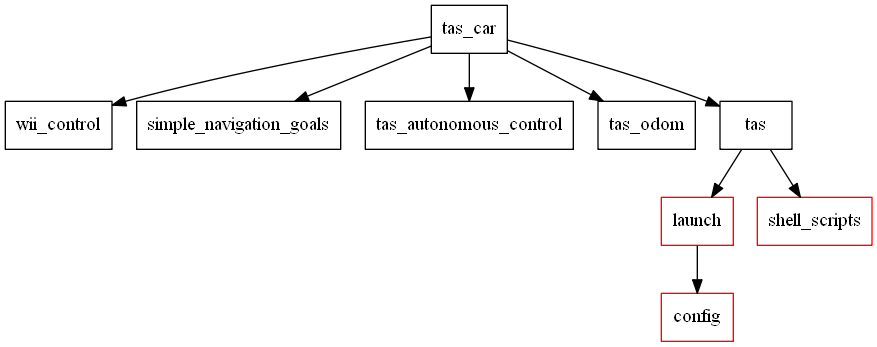
\includegraphics[width=\textwidth]{diagrams/tas_folder_struct}
	\caption{Folder structure of the TAS-package}
	\label{fig:tas_folder_struct}
\end{figure}

\newpage
\section{Installing the TAS-package}
\label{sec:tas_package_install 

As it was mentioned in the previous chapter the TAS-package can be found on GitHub. To install it open a terminal and switch to your catkin workspace directory. In this example we assume your working directory in \texttt{\textasciitilde/catkin\_ws}. To get and build the package on your car type in:

\shellcmd{cd \textasciitilde/catkin\_ws/src}\\
\shellcmd{git clone https://github.com/LSR-TAS/tas\_car}\\

To get the package running there are some preperations needed. Switch to the \texttt{shell\_scripts} folder and run the \texttt{ros\_setup.sh} script:

\shellcmd{cd \textasciitilde/catkin\_ws/src/tas\_car/tas/shell\_scripts}\\
\shellcmd{./ros\_setup.sh}\\

The script will take the following effects:

\begin{itemize}
\item Set rules for USB devices :\\
Usually Ubuntu names and numerates USB devices in a specific way. The numeration depends on the order in which the devices are plugged in. The script applies some rules to the system to assign clear names to the laserscanners and the arduino board.
\item Set up ROS environment:\\
Before working with ROS command line tools it is necessary to source a specific file. The script adds this command to the \texttt{~/.bashrc} file, which is executed each time you open a terminal. Therefore it is not required anymore to type in this command by hand. 
\end{itemize}

\textbf{After running the script, it is necessary to reboot the system.}

When the system has restarted it is ready to build the package. Open a terminal, switch to your catkin workspace and type:

\shellcmd{cd \textasciitilde/catkin\_ws}\\
\shellcmd{catkin\_make}\\

The package manager will now compile and build the code. If there occured no errors during the process the car is now ready to run! Before going on with the next section, please \textbf{reopen the terminal once}.

\newpage
\section{Hardware drivers}
\label{sec:tas_package_drivers}
The follwing section will show you how to run the hardware drivers on the car. After launching them it is already possible to drive the car around and control it manually with the wii controller.

\begin{figure}[h]
	\centering
		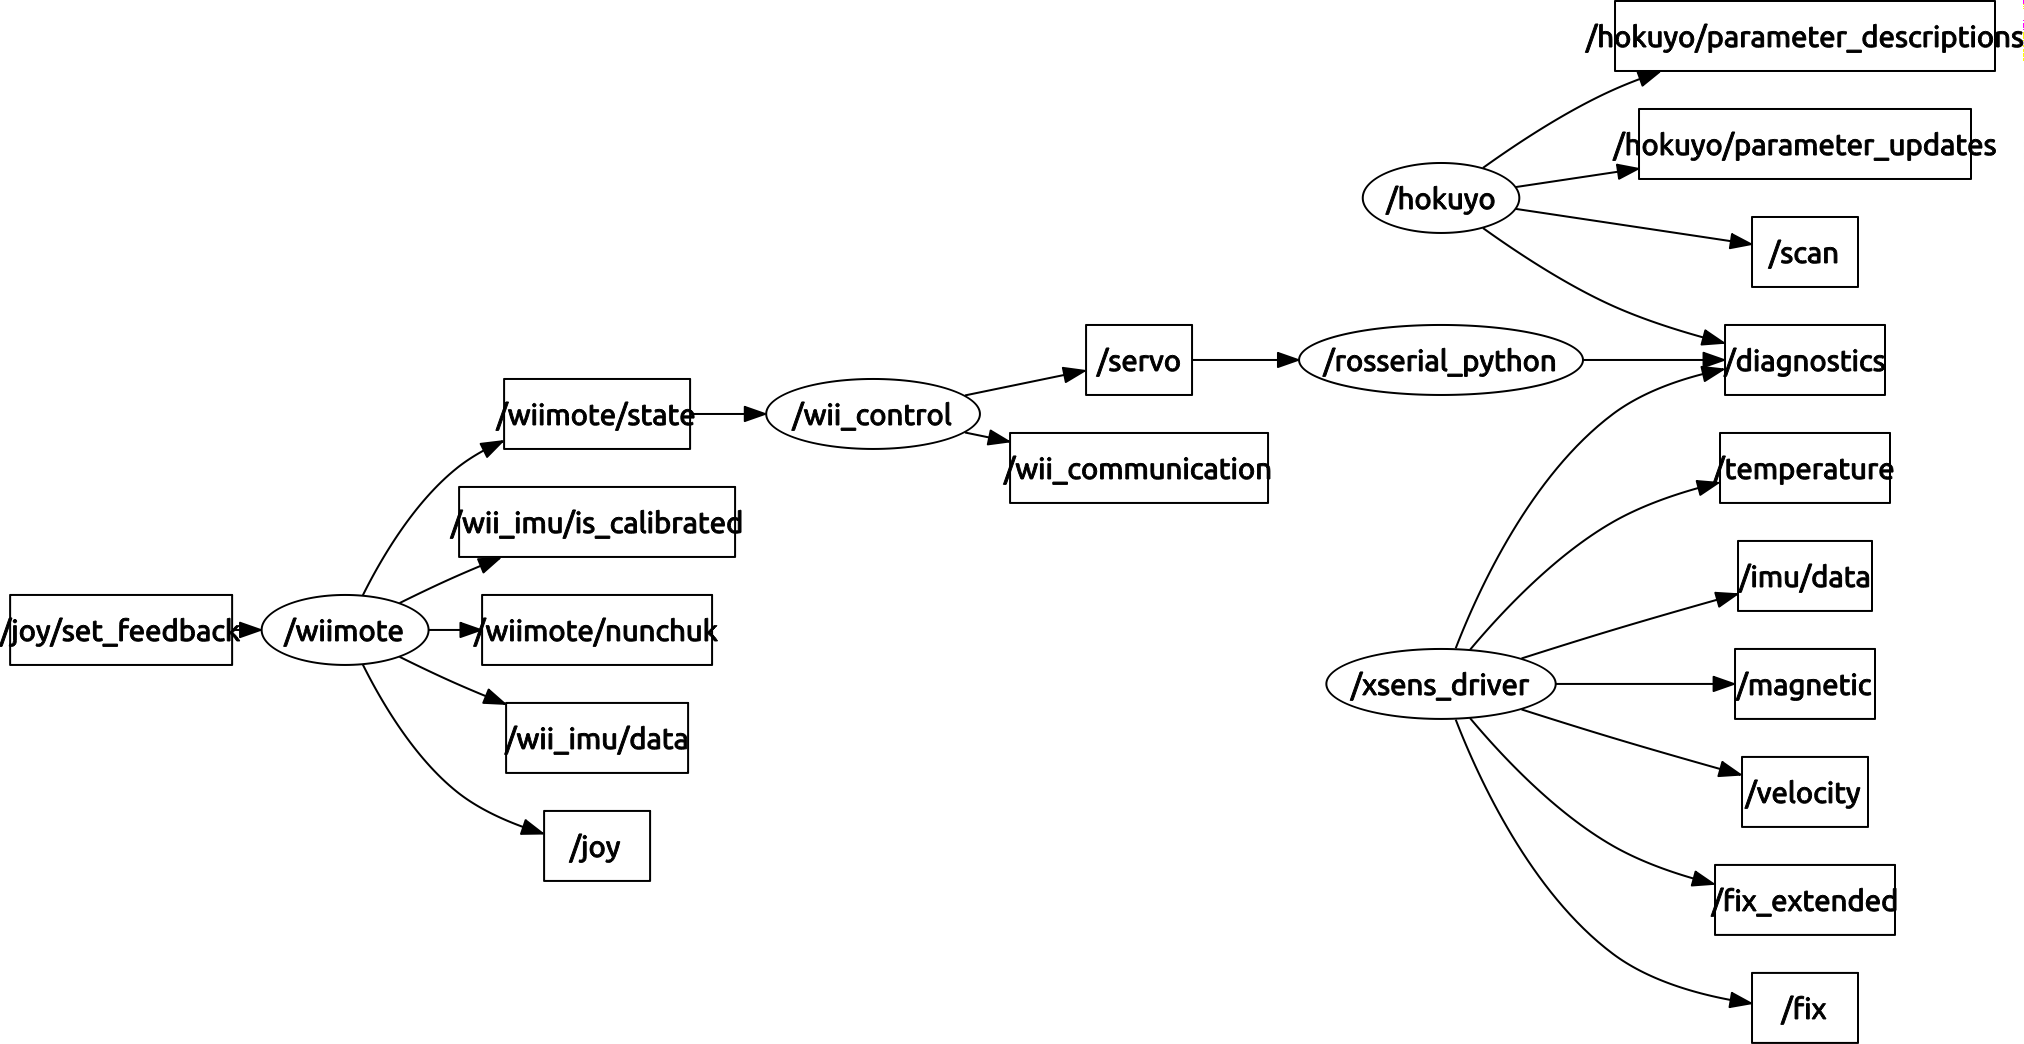
\includegraphics[width=0.9\textwidth]{diagrams/rqt_hardware}
	\caption{ROS nodes for the hardware}
	\label{fig:rqt_hardware}
\end{figure}

\begin{wrapfigure}{r}{0.13\textwidth}
  \begin{center}
    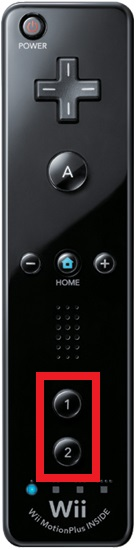
\includegraphics[width=0.13\textwidth]{wii}
		\caption{}
		\label{fig:wii_controller}
  \end{center}	
\end{wrapfigure}

To launch the hardware drivers open a terminal and type in:

\shellcmd{roscd tas/launch}\\
\shellcmd{roslaunch hardware.launch}

This will run several nodes to communicate with the hardware which will be explained in detail in the following sections. To establish the connection to the wii-controller press the the two two buttons at the bottom of the controller (see picture \reffig{wii_controller} on the right) for about 5 seconds until you see a notification in the terminal window. \textbf{If the motors are powered (see section \refsec{setup}), the car is now ready to run!}

In picture \reffig{rqt_hardware} you can see a graphical overview of the running nodes and topics. If you open a terminal and type in:

\shellcmd{rosrun rqt\_graph rqt\_graph}

you should get the same picture.


\subsection{wiimote}
\label{sec:tas_package_drivers_wiimote}
The \texttt{wiimote} node establishes a bluetooth connection to the wii-controller. It reads the inputs from the sticks and buttons of the controller and publishes these information to several ROS topics. Like you certainly have noticed, we use this data as control inputs for the car in manual mode. See the following link for a more detailed description:

\hyperref[http://wiki.ros.org/wiimote?distro=indigo]{http://wiki.ros.org/wiimote?distro=indigo}

\subsection{wii\_control}
\label{sec:tas_package_drivers_wii_control}
The motor controllers require a special PWM signal as control inputs (see picture \reffig{pwm_signals}). The \texttt{wii\_control} node takes the inputs from the wii-controller, calculates the corresponding PWM values and publises them to the \texttt{/servo} topic.


\subsection{rosserial\_python}
\label{sec:tas_package_drivers_rosserial}
The \texttt{rosserial\_python} node takes the PWM values from the \texttt{/servo} topic and sends them to the arduino via the USB port. It mainly implements the communication channel between nodes and topics over a (virtual) serial port. For correct communication there has to be installed the so called \texttt{rosserial\_client} on the arduino. For more information refer to:

\hyperref[http://wiki.ros.org/rosserial]{http://wiki.ros.org/rosserial}

\subsection{hokuyo\_node}
\label{sec:tas_package_drivers_hokuyo}
The \texttt{hokuyo\_node} is the driver for the laserscanner. It reads the measured data from the scanner via USB and publishes the to the \texttt{/scan} topic.

\hyperref[http://wiki.ros.org/hokuyo_node]{http://wiki.ros.org/hokuyo\_node}

\subsection{xsens\_driver}
\label{sec:tas_package_drivers_xsens}

The package provides a driver for several different IMUs from the XSens company. It reads data from the sensor via USB and publishes it to the \texttt{/imu/data} topic just like the \texttt{hokuyo\_node} does with the laser data.

\hyperref[http://wiki.ros.org/xsens_driver]{http://wiki.ros.org/xsens\_driver}

\newpage
\section{TAS-Odometry}
\label{sec:tas_package_odom}

\begin{figure}[h]
	\centering
		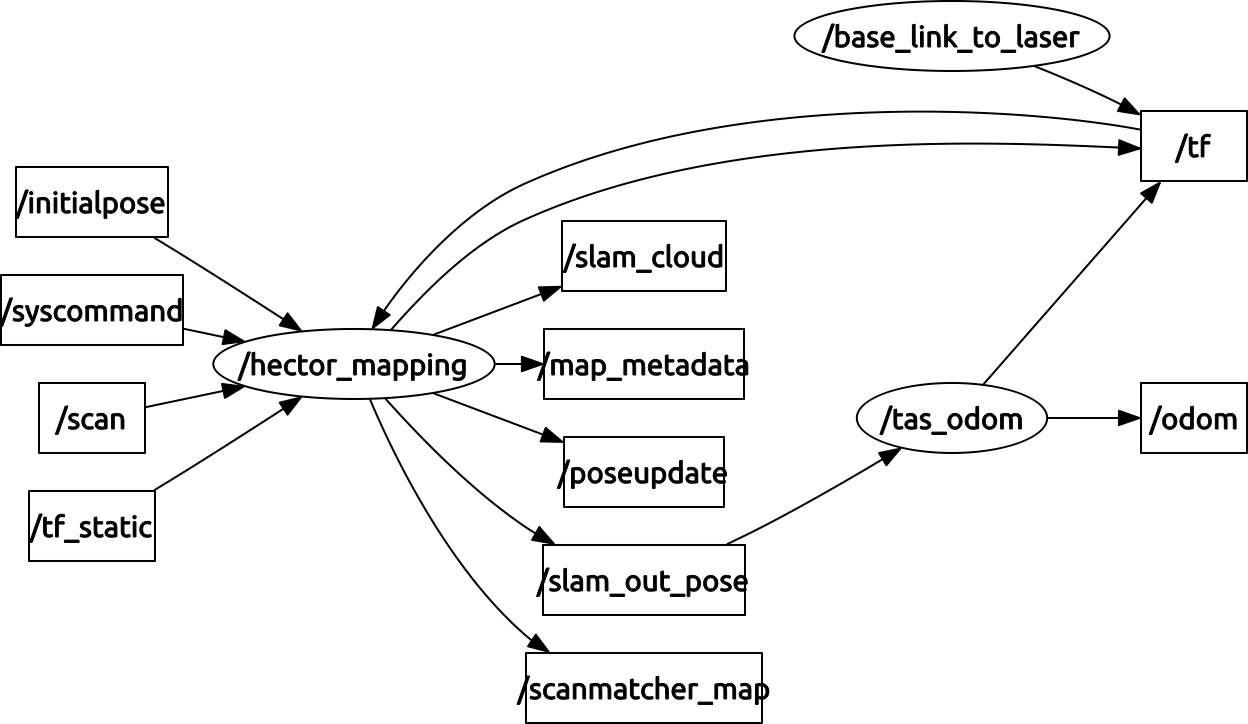
\includegraphics[width=0.9\textwidth]{diagrams/rqt_odom}
	\caption{Overview of the TAS-Odometry}
	\label{fig:rqt_odom}
\end{figure}

Currently there is no real odometry on the car available. For the navigation packages though odometry data is required (see picture \reffig{move_base_overview}). This was solved by using of a "fake-odometry". We take position and orientation estimated from the laserscanner data, and provide them as odometry data to the navigation package. 

To launch the fake odometry open a terminal and run the odom.launch file:

\shellcmd{roscd tas/launch} \\
\shellcmd{roslaunch odom.launch}

Picture \reffig{rqt_odom} shows the running nodes and topics for the fake odometry.

\subsection{hector\_mapping}
\label{sec:tas_package_odom_hector}

The hector\_mapping node implements a SLAM-algorithm \footnote{Simultaneous Localization and Mapping} to build a map and localize the car in it simultaneously at runtime. In picture \reffig{hector_buidling_process} you can see the building process. It shows the created map at three different timesteps.

\begin{figure}[h]
	\centering
		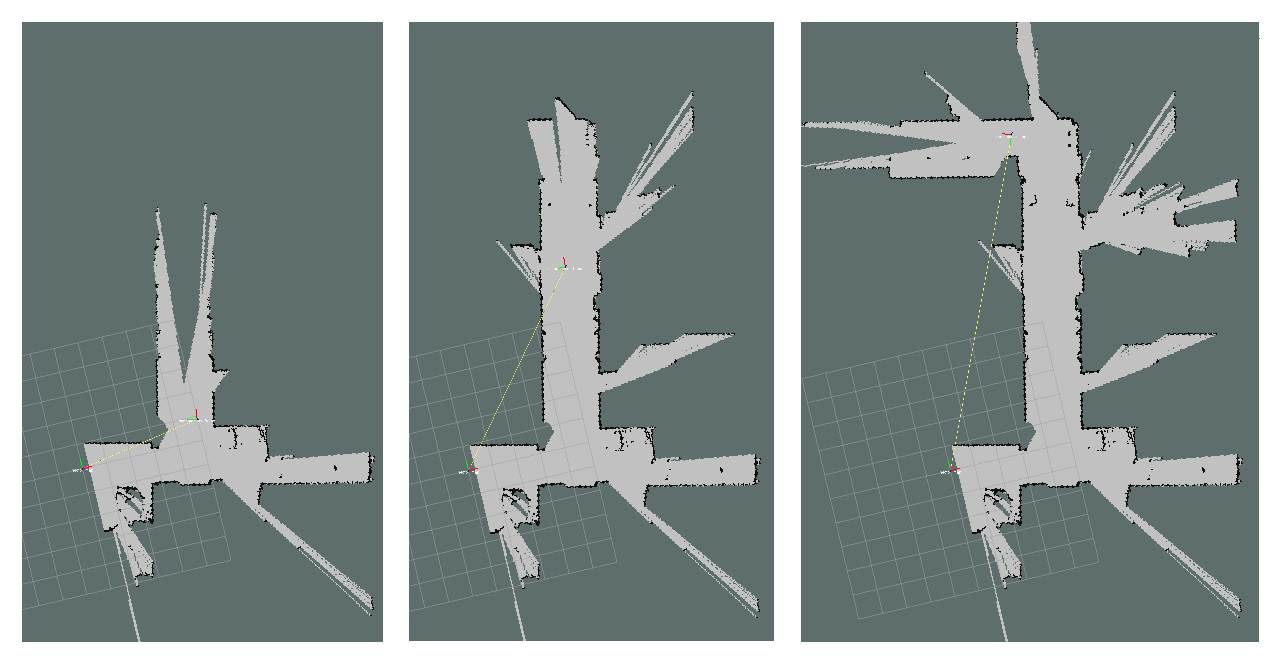
\includegraphics[width=\textwidth]{hector}
	\caption{Building process of a map with hector\_mapping}
	\label{fig:hector_buidling_process}
\end{figure}

Unlike other solutions for localization (see the \texttt{amcl package} in section \refsec{tas_package_amcl}) it only needs data from the laserscanner and does not require any odometry inputs. This is the reason why we use it to provide the fake odometry.

The estimated position and orientation is published to the \texttt{/poseupdate} (with covariance) and the \texttt{/slam\_out\_pose} topics (without covariance). 
 
For correct position estimation the node needs information about the relation between coordinate frame of the laserscanner and the coordinate frame of the car (refer to the next section \refsec{tas_package_transformations} for an introduction to transformations and frames). 

For more details about the parameters and settings of the package see:

\hyperref[http://wiki.ros.org/hector_mapping]{http://wiki.ros.org/hector\_mapping}

\section{Transformations}
\label{sec:tas_package_transformations}

\newpage
\section{Navigation}
\label{sec:tas_package_navigation}

\begin{figure}[h]
	\centering
		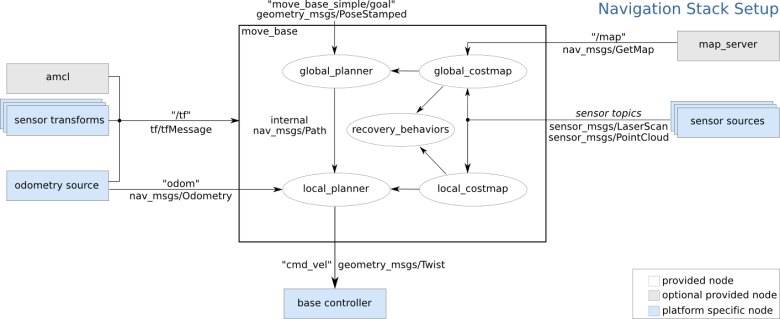
\includegraphics[width=\textwidth]{move_base_overview}
	\caption{Basic Navigation Stack}
	\label{fig:move_base_overview}
\end{figure}

In ROS in general the Navigation Stack takes sensor inputs from odometry, laser and other sources and outputs velocity commands to reach a given goal. Picture \reffig{move_base_overview} shows the parts of the basic Navigation Stack which is installed on the car.

To run the Navigation Stack open a terminal and type in:

\shellcmd{roscd tas/launch}\\
\shellcmd{roslaunch move\_base.launch}

The launch file will run all necessary parts of the Stack. Keep in mind that the hardware drivers and the TAS-Odometry package have to be launched before (see \refsec{tas_package_drivers} for hardware drivers and \refsec{tas_package_odom} for odometry).

To specify a goal for the car you can use the visualization tool RVIZ. Open a terminal and type in:

\shellcmd{roscd tas/launch} \\
\shellcmd{rosrun rviz rviz -d config/rviz/tas\_rviz.rviz}

This will run rviz with the configuration file in the \texttt{config} directory. At the beginning you have to give an initial estimation of the position to the \texttt{amcl node}. After that you can give goals to the \texttt{move\_base node} which the car will try to reach (see the marked buttons in picture \reffig{rviz_estimation}). To actually drive the car you have to push the \texttt{C-button} on the wii-nunchuk. 

\begin{figure}[h]
	\centering
		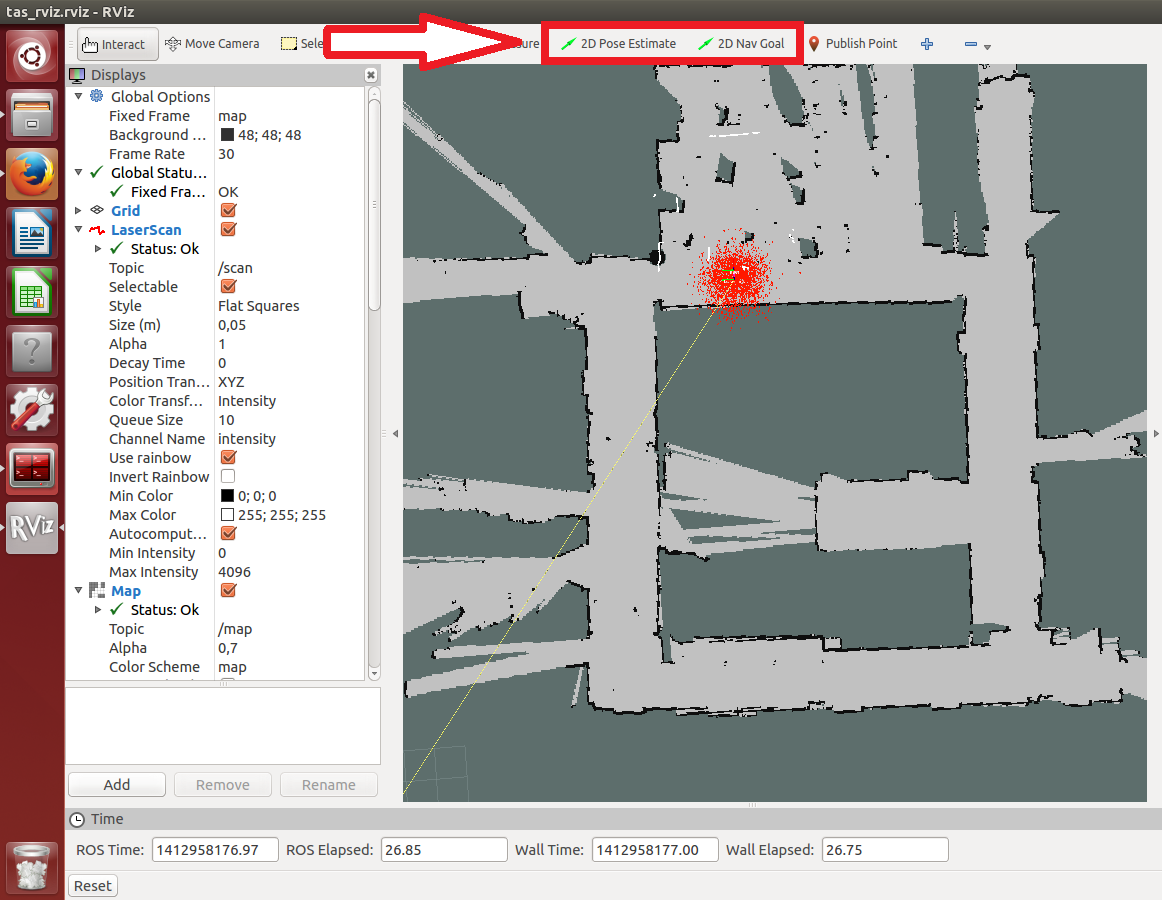
\includegraphics[width=\textwidth]{rviz_estimation}
	\caption{RVIZ visualization tool}
	\label{fig:rviz_estimation}
\end{figure}


Alternately you can launch hardware drivers, TAS-Odometry, the Navigation Stack and the RVIZ tool at once by launching the \texttt{run\_rviz.launch} file.

\subsection{map\_server}
\label{sec:tas_package_map_server}
The \texttt{map\_server} node takes a 2-D map of the environment and provides it as a ROS-service to other nodes. For every map there has to be a configuration file. The map file and the configuration file are located in the \texttt{config} directory of the TAS-package (see picture \reffig{tas_folder_struct} for the folder structure). The path of these files can be changed in the launchfile. For more information about the parameters of the \texttt{map\_server} package refer to:

\hyperref[http://wiki.ros.org/map_server]{http://wiki.ros.org/map\_server}


\subsection{amcl}
\label{sec:tas_package_amcl}
The \texttt{amcl} node implements different Monte Carlo localization algorithms to estimate the position of the robot. It requires a laserscanner, odometry and a map of the environment. The position and orientation with it's covariances is published to the \texttt{/amcl\_pose} topic.

The node takes odometry data in form of the transformation between the odometry frame and the coordinate frame of the car. See section \refsec{tas_package_transformations} for information about the \texttt{tf package}. Refer also to the package documentation on:

\hyperref[http://wiki.ros.org/amcl]{http://wiki.ros.org/amcl}



\subsection{move\_base}
\label{sec:tas_package_move_base}

The \texttt{mode\_base} implements a local and a global planner to calculate velocity commands to reach the navigation goal. These commands are published to the \texttt{/cmd\_vel} topic which is a general interface to the hardware of the robot. In our case the commands are taken by the \texttt{autonomous\_control} node to get the car moving (see next section \refsec{tas_package_autonomous_control}).

In the \texttt{config} folder (see picture \reffig{tas_folder_struct}) there are several configuration files for the planners. For information about settings and parameters refer to:

\hyperref[http://wiki.ros.org/move_base?distro=indigo]{http://wiki.ros.org/move\_base?distro=indigo}

\subsection{tas\_autonomous\_control}
\label{sec:tas_package_autonomous_control}
The  \texttt{autonomous\_control} node mainly takes the velocity commands generated by the \texttt{move\_base} node and publishes the corresponding PWM values for the motor controllers to the \texttt{/servo} topic.

For safety reasons the car only drives autonomously if the \texttt{C-button} on the wii-nunchuk is pressed.

Pay attention, that currently there are only two discrete velocity states implemented. See the following extract from the source code of the node:

\begin{lstlisting}
if(autonomous_control.cmd_linearVelocity>0) {
	autonomous_control.control_servo.x = 1550;
}

else if(autonomous_control.cmd_linearVelocity<0) {
	autonomous_control.control_servo.x = 1300;
}

else {
	autonomous_control.control_servo.x = 1500;
}

autonomous_control.control_servo.y = 
 autonomous_control.cmd_steeringAngle;
\end{lstlisting}











